%插入样式内容
\documentclass[12pt]{article}
%%---------------------------------------------------------------------
% packages
% geometry
\usepackage{geometry}
% font
\usepackage{fontspec}
\defaultfontfeatures{Mapping=tex-text}  %%如果没有它,会有一些 tex 特殊字符无法正常使用,比如连字符。
\usepackage{xunicode,xltxtra}
\usepackage[BoldFont,SlantFont,CJKnumber,CJKchecksingle]{xeCJK}  % \CJKnumber{12345}: 一万二千三百四十五
\usepackage{CJKfntef}  %%实现对汉字加点、下划线等。
\usepackage{pifont}  % \ding{}
% math
\usepackage{amsmath,amsfonts,amssymb}
% color
\usepackage{color}
\usepackage{xcolor}
\definecolor{EYE}{RGB}{199,237,204}
\definecolor{FLY}{RGB}{128,0,128}
\definecolor{ZHY}{RGB}{139,0,255}
% graphics
\usepackage[americaninductors,europeanresistors]{circuitikz}
\usepackage{tikz}
\usetikzlibrary{positioning,arrows,shadows,shapes,calc,mindmap,trees,backgrounds}  % placements=positioning
\usepackage{graphicx}  % \includegraphics[]{}
\usepackage{subfigure}  %%图形或表格并排排列
% table
\usepackage{colortbl,dcolumn}  %% 彩色表格
\usepackage{multirow}
\usepackage{multicol}
\usepackage{booktabs}
% code
\usepackage{fancyvrb}
\usepackage{listings}
% title
\usepackage{titlesec}
% head/foot
\usepackage{fancyhdr}
% ref
\usepackage{hyperref}
% pagecolor
\usepackage[pagecolor={EYE}]{pagecolor}
% tightly-packed lists
\usepackage{mdwlist}

\usepackage{styles/iplouccfg}
\usepackage{styles/zhfontcfg}
\usepackage{styles/iplouclistings}

\usepackage{color,framed}

%%---------------------------------------------------------------------
% settings
% geometry
\geometry{left=2cm,right=1cm,top=2cm,bottom=2cm}  %设置 上、左、下、右 页边距
\linespread{1.5} %行间距
% font
\setCJKmainfont{Adobe Kaiti Std}
%\setmainfont[BoldFont=Adobe Garamond Pro Bold]{Apple Garamond}  % 英文字体
%\setmainfont[BoldFont=Adobe Garamond Pro Bold,SmallCapsFont=Apple Garamond,SmallCapsFeatures={Scale=0.7}]{Apple Garamond}  %%苹果字体没有SmallCaps
\setCJKmonofont{Adobe Fangsong Std}
% graphics
\graphicspath{{figures/}}
\tikzset{
    % Define standard arrow tip
    >=stealth',
    % Define style for boxes
    punkt/.style={
           rectangle,
           rounded corners,
           draw=black, very thick,
           text width=6.5em,
           minimum height=2em,
           text centered},
    % Define arrow style
    pil/.style={
           ->,
           thick,
           shorten <=2pt,
           shorten >=2pt,},
    % Define style for FlyZhyBall
    FlyZhyBall/.style={
      circle,
      minimum size=6mm,
      inner sep=0.5pt,
      ball color=red!50!blue,
      text=white,},
    % Define style for FlyZhyRectangle
    FlyZhyRectangle/.style={
      rectangle,
      rounded corners,
      minimum size=6mm,
      ball color=red!50!blue,
      text=white,},
    % Define style for zhyfly
    zhyfly/.style={
      rectangle,
      rounded corners,
      minimum size=6mm,
      ball color=red!25!blue,
      text=white,},
    % Define style for new rectangle
    nrectangle/.style={
      rectangle,
      draw=#1!50,
      fill=#1!20,
      minimum size=5mm,
      inner sep=0.1pt,}
}
\ctikzset{
  bipoles/length=.8cm
}
% code
\lstnewenvironment{VHDLcode}[1][]{%
  \lstset{
    basicstyle=\footnotesize\ttfamily\color{black},%
    columns=flexible,%
    framexleftmargin=.7mm,frame=shadowbox,%
    rulesepcolor=\color{blue},%
%    frame=single,%
    backgroundcolor=\color{yellow!20},%
    xleftmargin=1.2\fboxsep,%
    xrightmargin=.7\fboxsep,%
    numbers=left,numberstyle=\tiny\color{blue},%
    numberblanklines=false,numbersep=7pt,%
    language=VHDL%
    }\lstset{#1}}{}
\lstnewenvironment{VHDLmiddle}[1][]{%
  \lstset{
    basicstyle=\scriptsize\ttfamily\color{black},%
    columns=flexible,%
    framexleftmargin=.7mm,frame=shadowbox,%
    rulesepcolor=\color{blue},%
%    frame=single,%
    backgroundcolor=\color{yellow!20},%
    xleftmargin=1.2\fboxsep,%
    xrightmargin=.7\fboxsep,%
    numbers=left,numberstyle=\tiny\color{blue},%
    numberblanklines=false,numbersep=7pt,%
    language=VHDL%
    }\lstset{#1}}{}
\lstnewenvironment{VHDLsmall}[1][]{%
  \lstset{
    basicstyle=\tiny\ttfamily\color{black},%
    columns=flexible,%
    framexleftmargin=.7mm,frame=shadowbox,%
    rulesepcolor=\color{blue},%
%    frame=single,%
    backgroundcolor=\color{yellow!20},%
    xleftmargin=1.2\fboxsep,%
    xrightmargin=.7\fboxsep,%
    numbers=left,numberstyle=\tiny\color{blue},%
    numberblanklines=false,numbersep=7pt,%
    language=VHDL%
    }\lstset{#1}}{}
% pdf
\hypersetup{%pdfpagemode=FullScreen,%
            pdfauthor={Haiyong Zheng},%
            pdftitle={Title},%
            CJKbookmarks=true,%
            bookmarksnumbered=true,%
            bookmarksopen=false,%
            plainpages=false,%
            colorlinks=true,%
            citecolor=green,%
            filecolor=magenta,%
            linkcolor=cyan,%red(default)
            urlcolor=cyan}
% section
%http://tex.stackexchange.com/questions/34288/how-to-place-a-shaded-box-around-a-section-label-and-name
\newcommand\titlebar{%
\tikz[baseline,trim left=3.1cm,trim right=3cm] {
    \fill [cyan!25] (2.5cm,-1ex) rectangle (\textwidth+3.1cm,2.5ex);
    \node [
        fill=cyan!60!white,
        anchor= base east,
        rounded rectangle,
        minimum height=3.5ex] at (3cm,0) {
        \textbf{\thesection.}
    };
}%
}
\titleformat{\section}{\Large\bf\color{blue}}{\titlebar}{0.1cm}{}
% head/foot
\setlength{\headheight}{15pt}
\pagestyle{fancy}
\fancyhf{}

\chead{\color{black!50!green}DIGITS DevBox}

%\lfoot{\color{blue!50!green}Dai Jialun}
\cfoot{\color{blue!50!green}\href{http://vision.ouc.edu.cn/~zhenghaiyong}{CVBIOUC}}
\rfoot{\color{blue!50!green}$\cdot$\ \thepage\ $\cdot$}
\renewcommand{\headrulewidth}{0.4pt}
\renewcommand{\footrulewidth}{0.4pt}


%%---------------------------------------------------------------------
\begin{document}
%%---------------------------------------------------------------------
%%---------------------------------------------------------------------
% \titlepage
\title{\vspace{-2em} DIGITS\_DevBox深度学习服务器\\
\normalsize{}}
\author{Dai Jialun}
\date{\vspace{-0.7em} \today \vspace{-0.7em}}
%%---------------------------------------------------------------------
\maketitle\thispagestyle{fancy}
%%---------------------------------------------------------------------
\maketitle
%\tableofcontents 
\section{硬件配置}
\begin{description}
\item[显卡] 4个ASUS(华硕)GTX 980Ti-6GD5
\item[CPU] 1个Intel(英特尔) Core i7-5960X
\item[主板] 1个ASUS(华硕)X99-E WS
\item[内存] 2个CORSAIR(海盗船) VENGERNCE(复仇者)LPX 32GB(4 $\times$ 8GB) DDR4 2400MHz CMK32GX4M4A2400C14R
\item[硬盘] 3个WesternDigital(西部数码) 4TB 7200转
\item[固态硬盘] 1个Samsung(三星)SSD 850pro 512GB
\item[固态硬盘 for RAID] 1个Samsung SSD 512GB SM951
\item[机箱] 1个CORSAIR(海盗船) 900D
\item[电源] 1个CORSAIR(海盗船) AX1500i 1500W
\item[散热器] 1个CORSAIR(海盗船) H110 水冷CPU散热器
\item[风扇] 6个CORSAIR(海盗船)AF120 静音版 双包装
\item[光驱] 1个AUSU(华硕)DRW-24D1ST
\item[配件] 1个Thermaltake Commander FT触控式面板风扇控制器,Deepcool FAN HUB(九州风神风扇集线器)
\item[显示器]
\item[键盘鼠标]
\end{description}

\section{名词解释}
\begin{description}

\item[DVI] Digital Visual Interface,数字视频接口
\begin{figure}[!h]
\centering
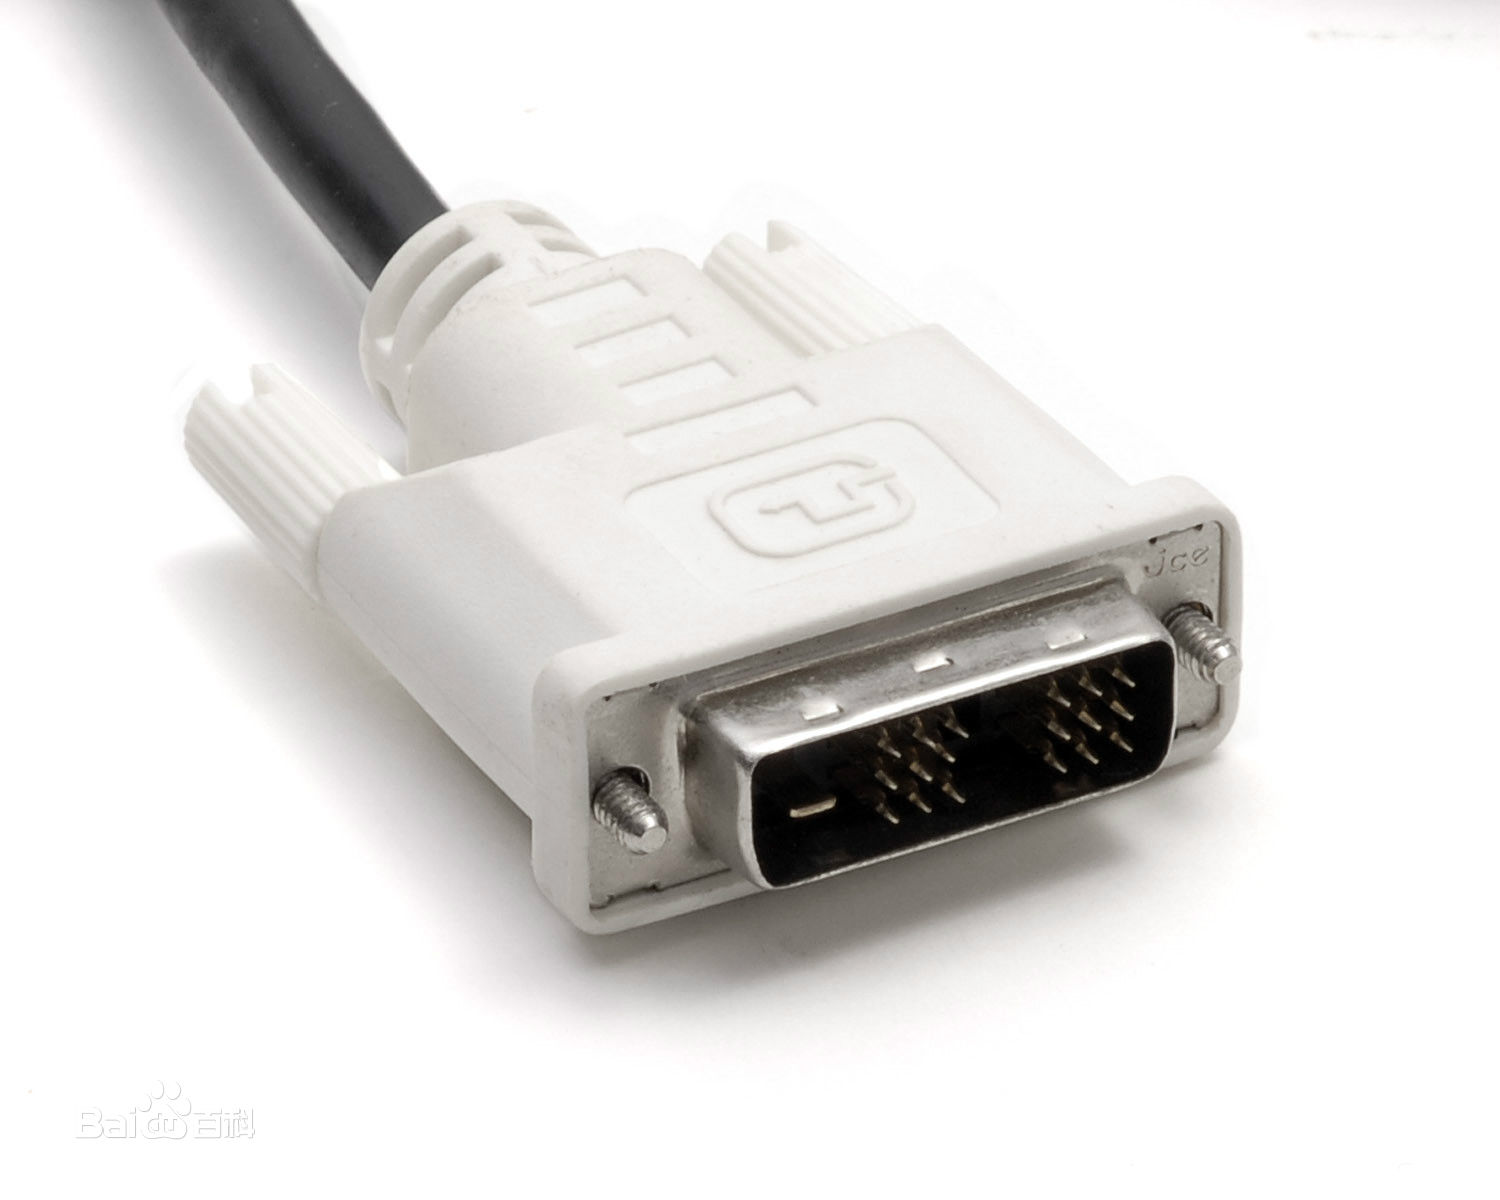
\includegraphics[width=0.2\textwidth]{DVI}
\end{figure}

\item[DislayPort] 高清数字显示借口标准
\begin{figure}[!ht]
\centering
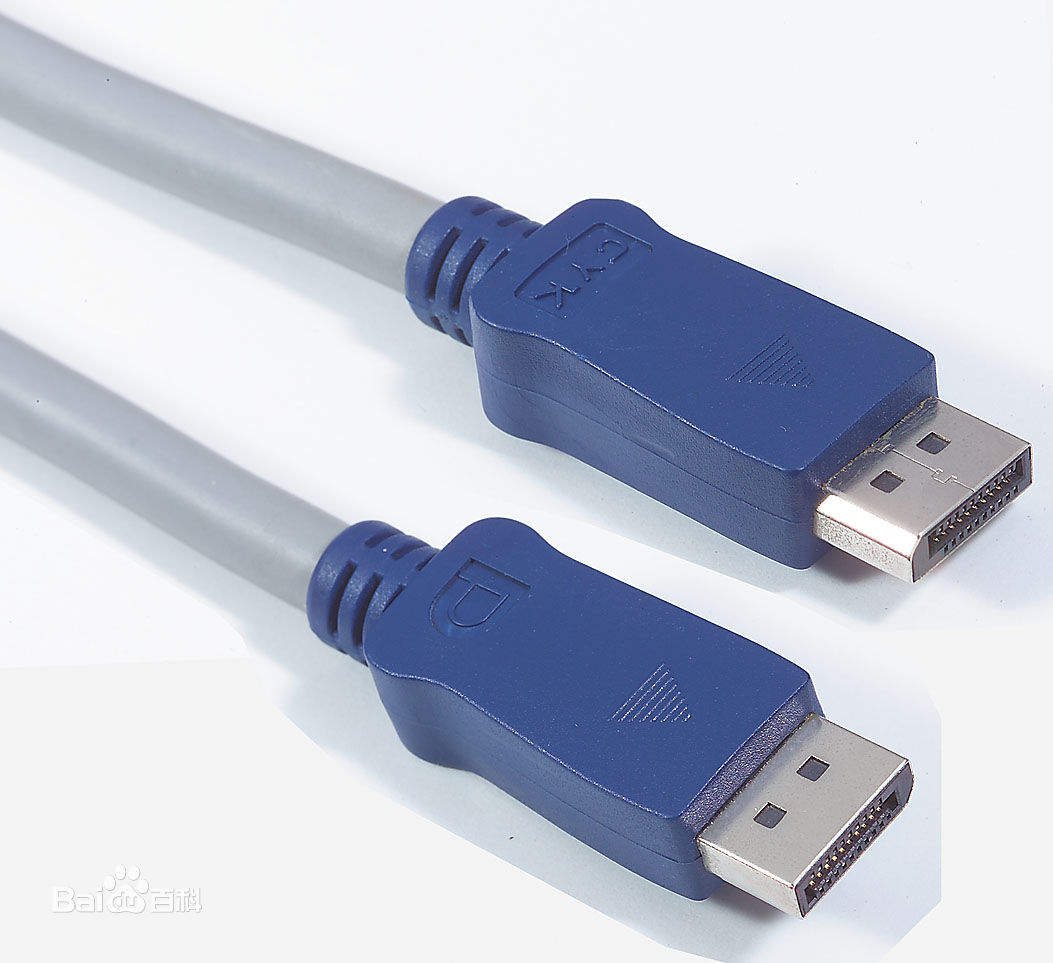
\includegraphics[width=0.2\textwidth]{DisplayPort}
\end{figure}

\item[PCI-E] PCI Express,新的总线接口
\begin{figure}[!ht]
\centering
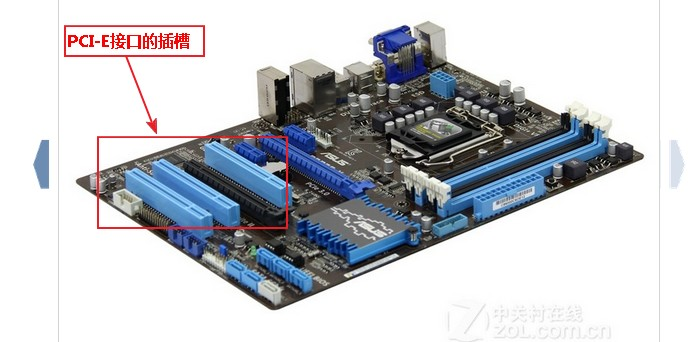
\includegraphics[width=0.2\textwidth]{PCI-E}
\end{figure}

\item[SATA Revision 3.0] Serial Advanced Technology Attachment,串行ATA规格第三版,6Gbps
\begin{figure}[!ht]
\centering
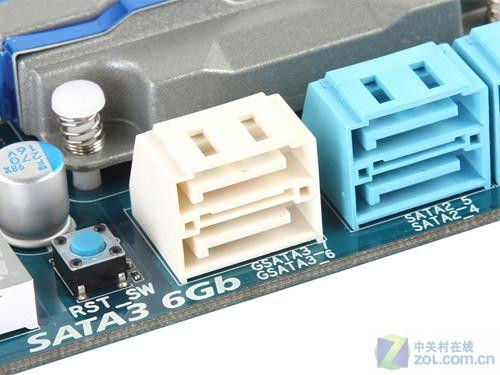
\includegraphics[width=0.2\textwidth]{SATA3}
\end{figure}

\item[SATA EXpress] SATA 3.0下一代的SATA接口,10Gbps
\begin{figure}[!ht]
\centering
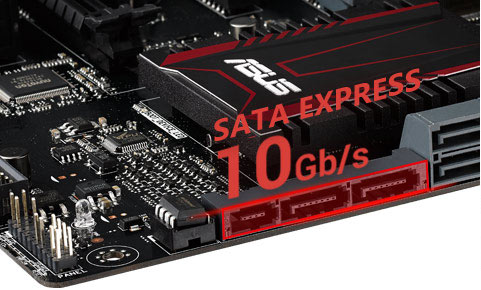
\includegraphics[width=0.2\textwidth]{SATAE}
\end{figure}

\item[M.2] 一种替代MSATA新的接口规范,优势体现在速度和体积。支持Socket2和Socket3两种接口类型
\begin{figure}[!ht]
  \centering 
  \subfigure[]{ 
    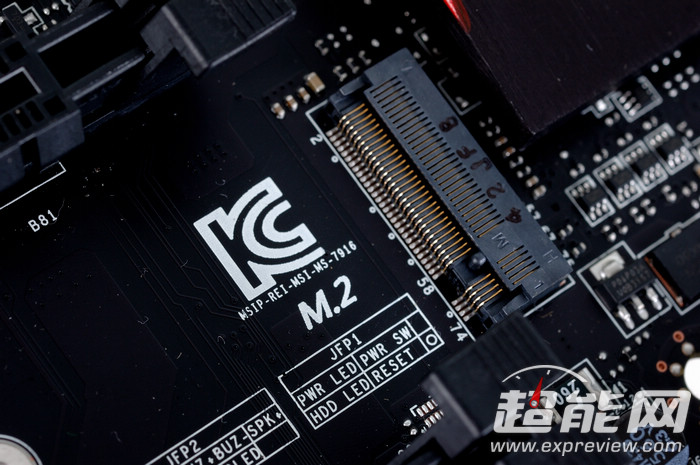
\includegraphics[width=0.23\textwidth]{M2}} 
  \subfigure[]{ 
    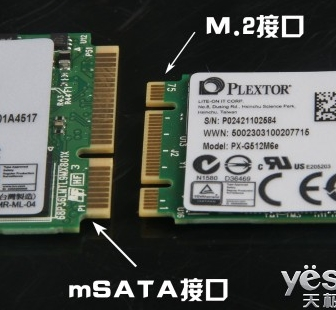
\includegraphics[width=0.17\textwidth]{M2-MSATA}} 
  \caption{}
\end{figure}

\item[RAID] Redundant Arrays of Independent Disks,磁盘阵列。磁盘阵列是由很多价格较便宜的磁盘,组合成一个容量巨大的磁盘组,利用个别磁盘提供数据所产生加成效果提升整个磁盘系统效能。利用这项技术,将数据切割成许多区段,分别存放在各个硬盘上。
\begin{figure}[!ht]
  \centering 
  \subfigure[]{ 
    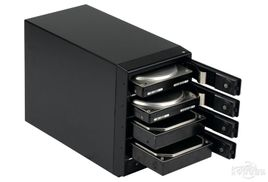
\includegraphics[width=0.24\textwidth]{RAID1}} 
  \subfigure[]{ 
    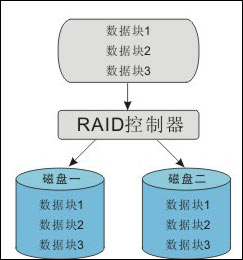
\includegraphics[width=0.15\textwidth]{RAID2}} 
  \caption{}
\end{figure}

\item[RAID] 一种存储性能、数据安全和存储成本兼顾的存储解决方案。为系统提供数据安全保障,但保障程度要比Mirror低而磁盘空间利用率要比Mirror高。数据以块为单位分布到各个硬盘上。RAID 5不对数据进行备份,而是把数据和与其相对应的奇偶校验信息存储到组成RAID5的各个磁盘上,并且奇偶校验信息和相对应的数据分别存储于不同的磁盘上。当RAID5的一个磁盘数据损坏后,利用剩下的数据和相应的奇偶校验信息去恢复被损坏的数据。
\begin{figure}[!ht]
\centering
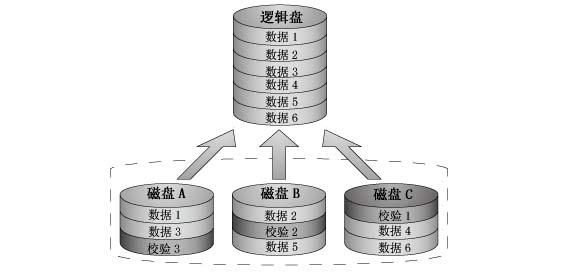
\includegraphics[width=0.4\textwidth]{RAID5}
\end{figure}

\item[SLI] Scalable Link Interface,可灵活伸缩的连接接口(支持多显卡技术)。这是一种可把两张或以上的显卡连在一起,作单一输出使用的技术,从而达至绘图处理效能加强的效果。
\begin{figure}[!ht]
\centering
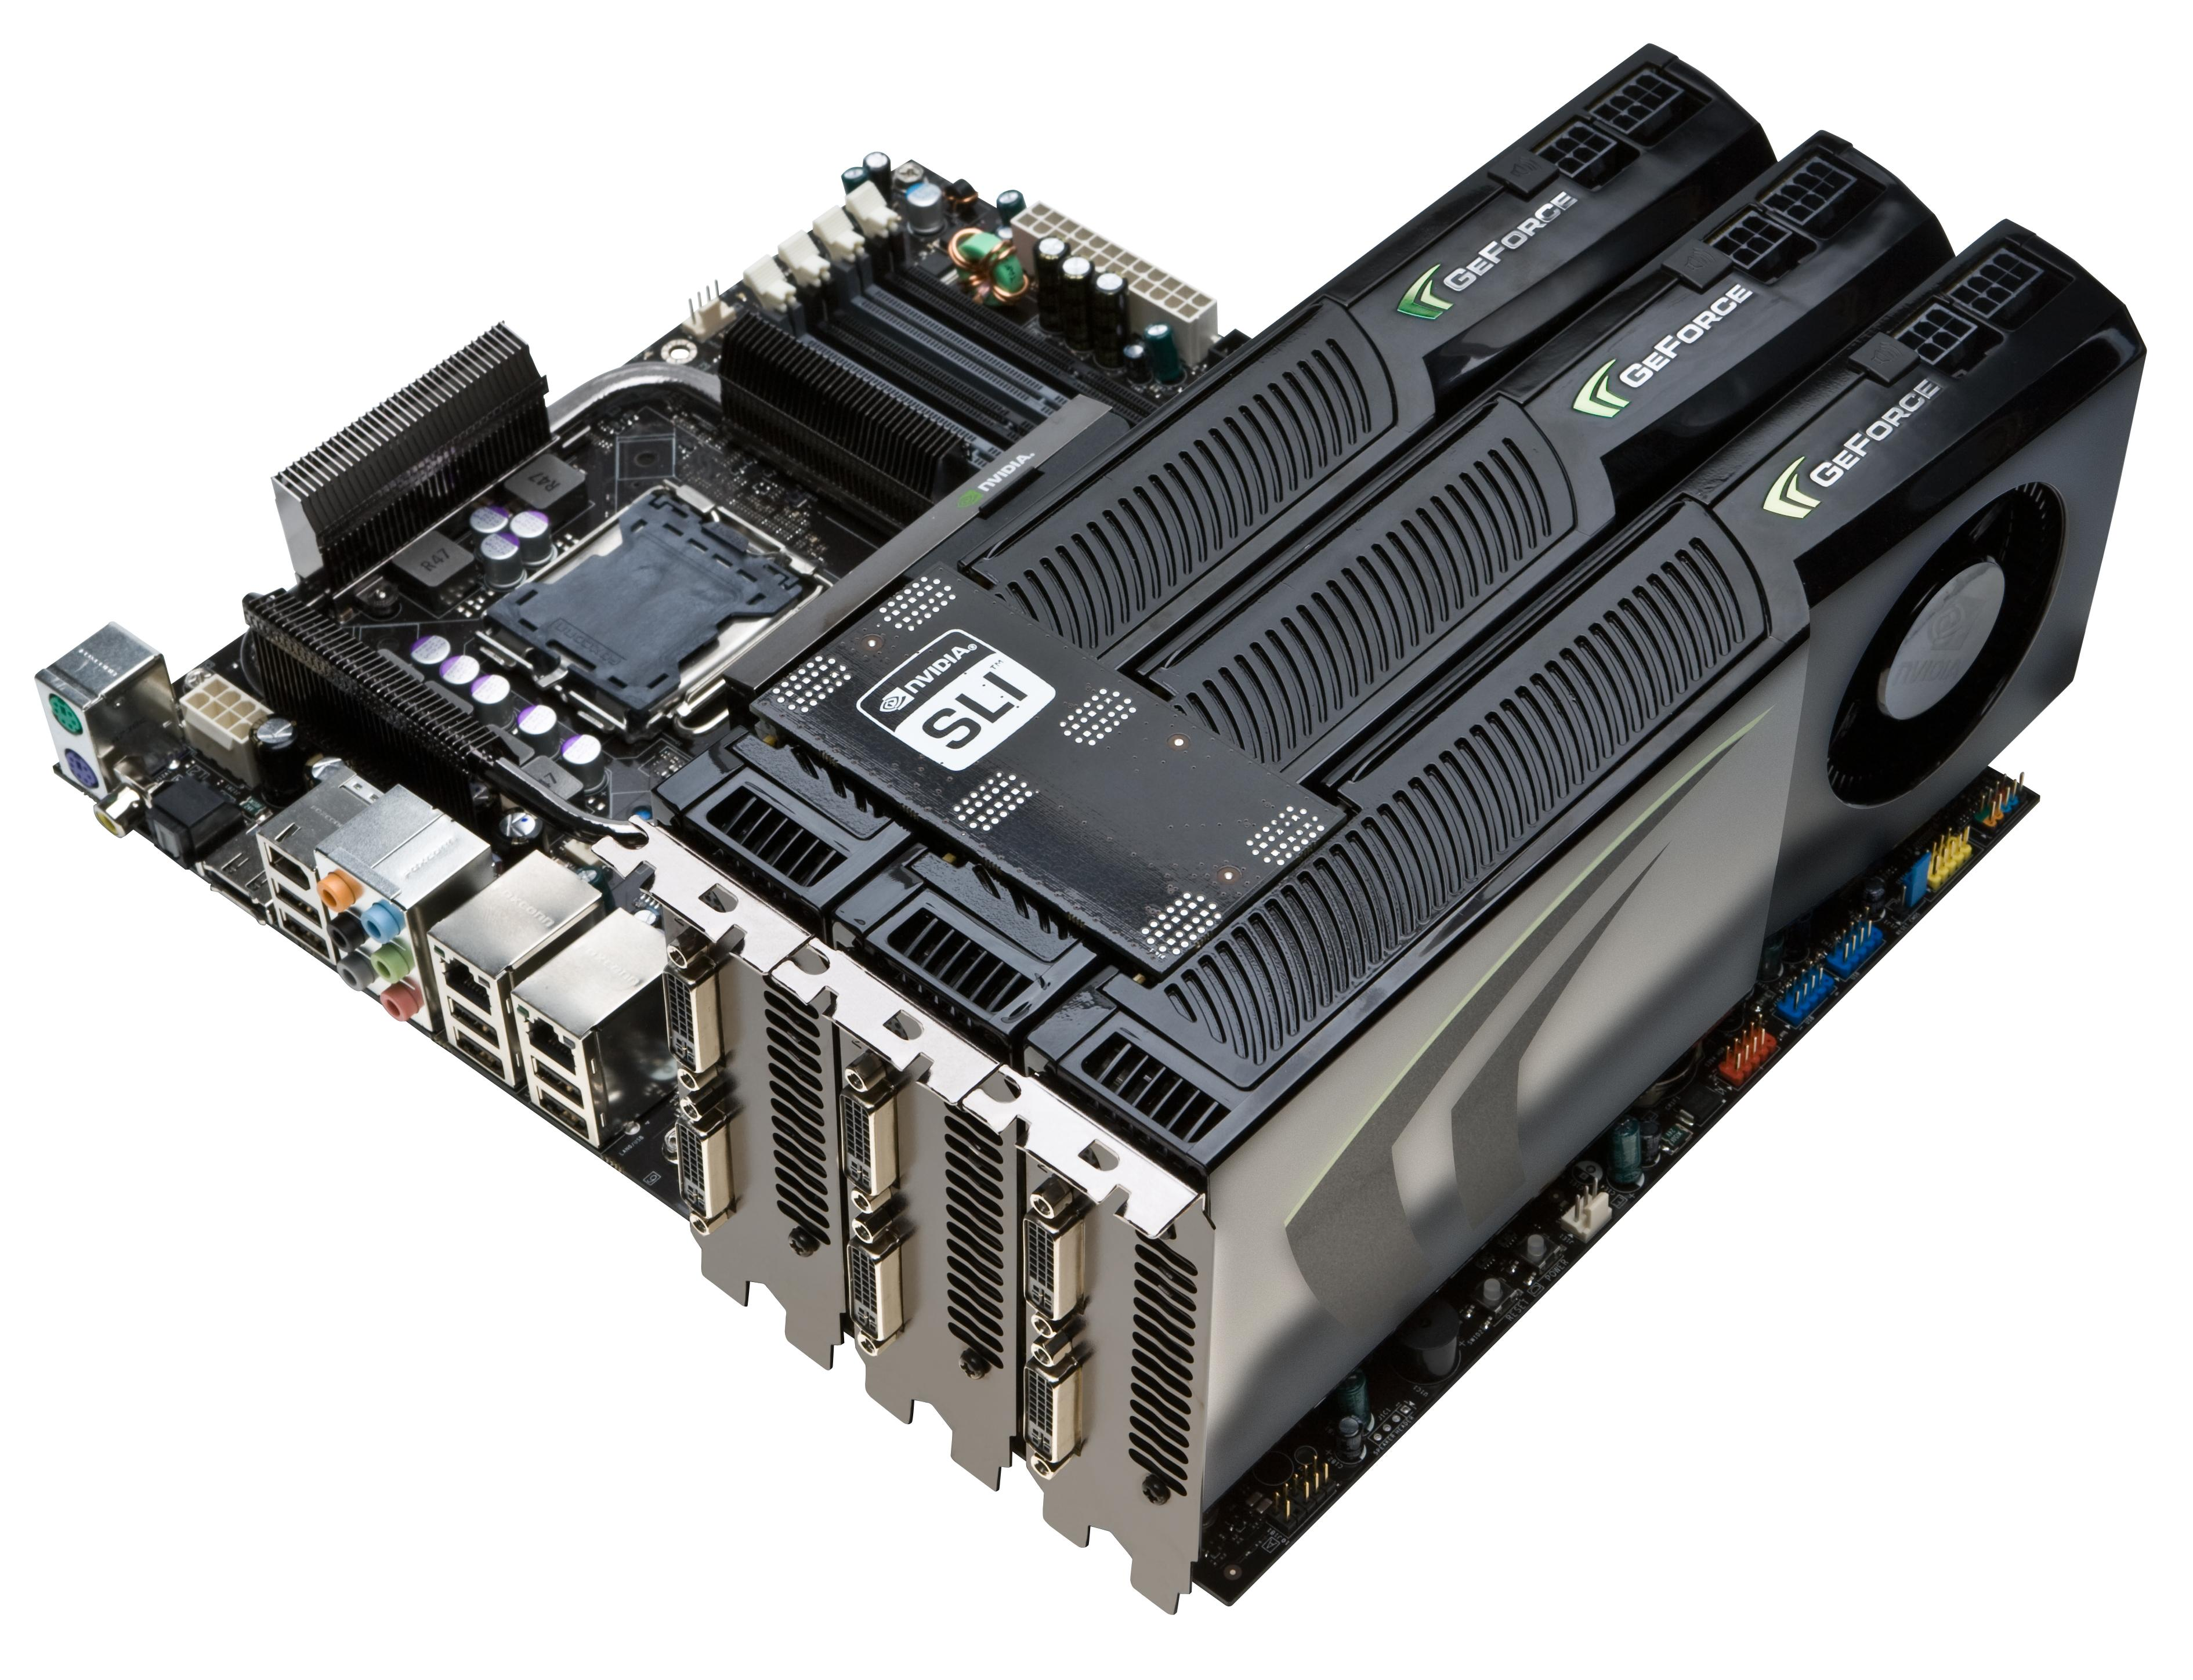
\includegraphics[width=0.2\textwidth]{SLI}
\end{figure}

\item[DDR4] Dual Data Rate SDRAM,是一种高速CMOS动态随即访问的内存。DDR4支持2133MHz,32GB DDR4-2133达到48.4GB/s。

\item[GDDR5] Graphics Double Data Rate SDRAM version5,是一种高性能显卡用内存,需搭配支持PCI-E以上规格的显卡,高频率达4GHZ,低功耗。
\end{description}
%%---------------------------------------------------------------------
\end{document}
